\documentclass[thesis.tex]{subfiles}

\chapter{Thử nghiệm và đánh giá}
\section{Dữ liệu}

\subsubsection{Dữ liệu nguồn và dữ liệu đích}

Dữ liệu chính được sử dụng trong đồ án này là GTA5 \cite{murez2018image} và Cityscapes \cite{cordts2015cityscapes}. 

Trong đó, bộ dữ liệu GTA5 chứa 24966 hình ảnh tổng hợp với chú thích ngữ nghĩa tới từng điểm ảnh được chia thành 10 tập nhỏ, mỗi tập 2500 ảnh ngoại trừ tập cuối có 2466 ảnh. Các hình ảnh đã được kết xuất bằng cách sử dụng trò chơi điện tử thế giới mở Grand Theft Auto 5 và tất cả đều từ góc nhìn xe hơi trên đường phố của các thành phố ảo theo phong cách Mỹ. Có 19 lớp ngữ nghĩa tương thích với các lớp trong bộ dữ liệu Cityscapes (Hình \ref{fig:gta5}).

\begin{figure}[htp]
	\centering
	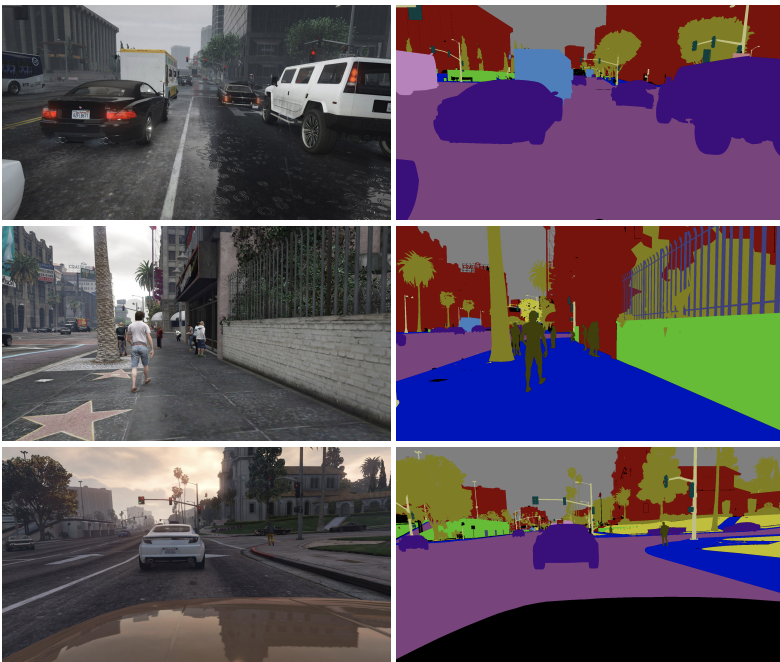
\includegraphics[width=0.6\textwidth]{images/gta5.png}
	\caption{Dữ liệu trong GTA5 được trích xuất từ trò chơi điện tử}
	\label{fig:gta5}
\end{figure}
% \FloatBarrier

Bên cạnh đó, bộ dữ liệu Cityscapes tập trung vào cảnh đường phố đô thị. Tập dữ liệu bao gồm 30 lớp ngữ nghĩa được chụp từ góc nhìn của xe hơi tại 50 thành phố trên kháp thế giới trải dài qua các tháng trong năm. Cityscapes bao gồm 5000 ảnh với nhãn tinh và 20000 ảnh với nhãn thô. Đồ án này chỉ sử dụng 5000 ảnh với nhãn tinh và kiểm thử trên tập dữ liệu với 500 ảnh.

Các đối tượng cần nhận diện được gắn nhãn không được có những mảng đen, tức là nếu có một số hậu cảnh có thể nhìn thấy ‘xuyên qua’ đối tượng nào đó, nó được coi là một phần của đối tượng đó luôn. Điều này cũng áp dụng cho các vùng có nhiều hỗn hợp với hai hoặc nhiều lớp: chúng được gắn nhãn với lớp nằm phía trước. Ví dụ: cây lá trước cửa nhà hoặc bầu trời (mọi thứ thuộc về cây), cửa sổ ô tô trong suốt (mọi thứ thuộc về ô tô) (Hình \ref{fig:cityscapes}).

\begin{figure}[htp]
	\centering
	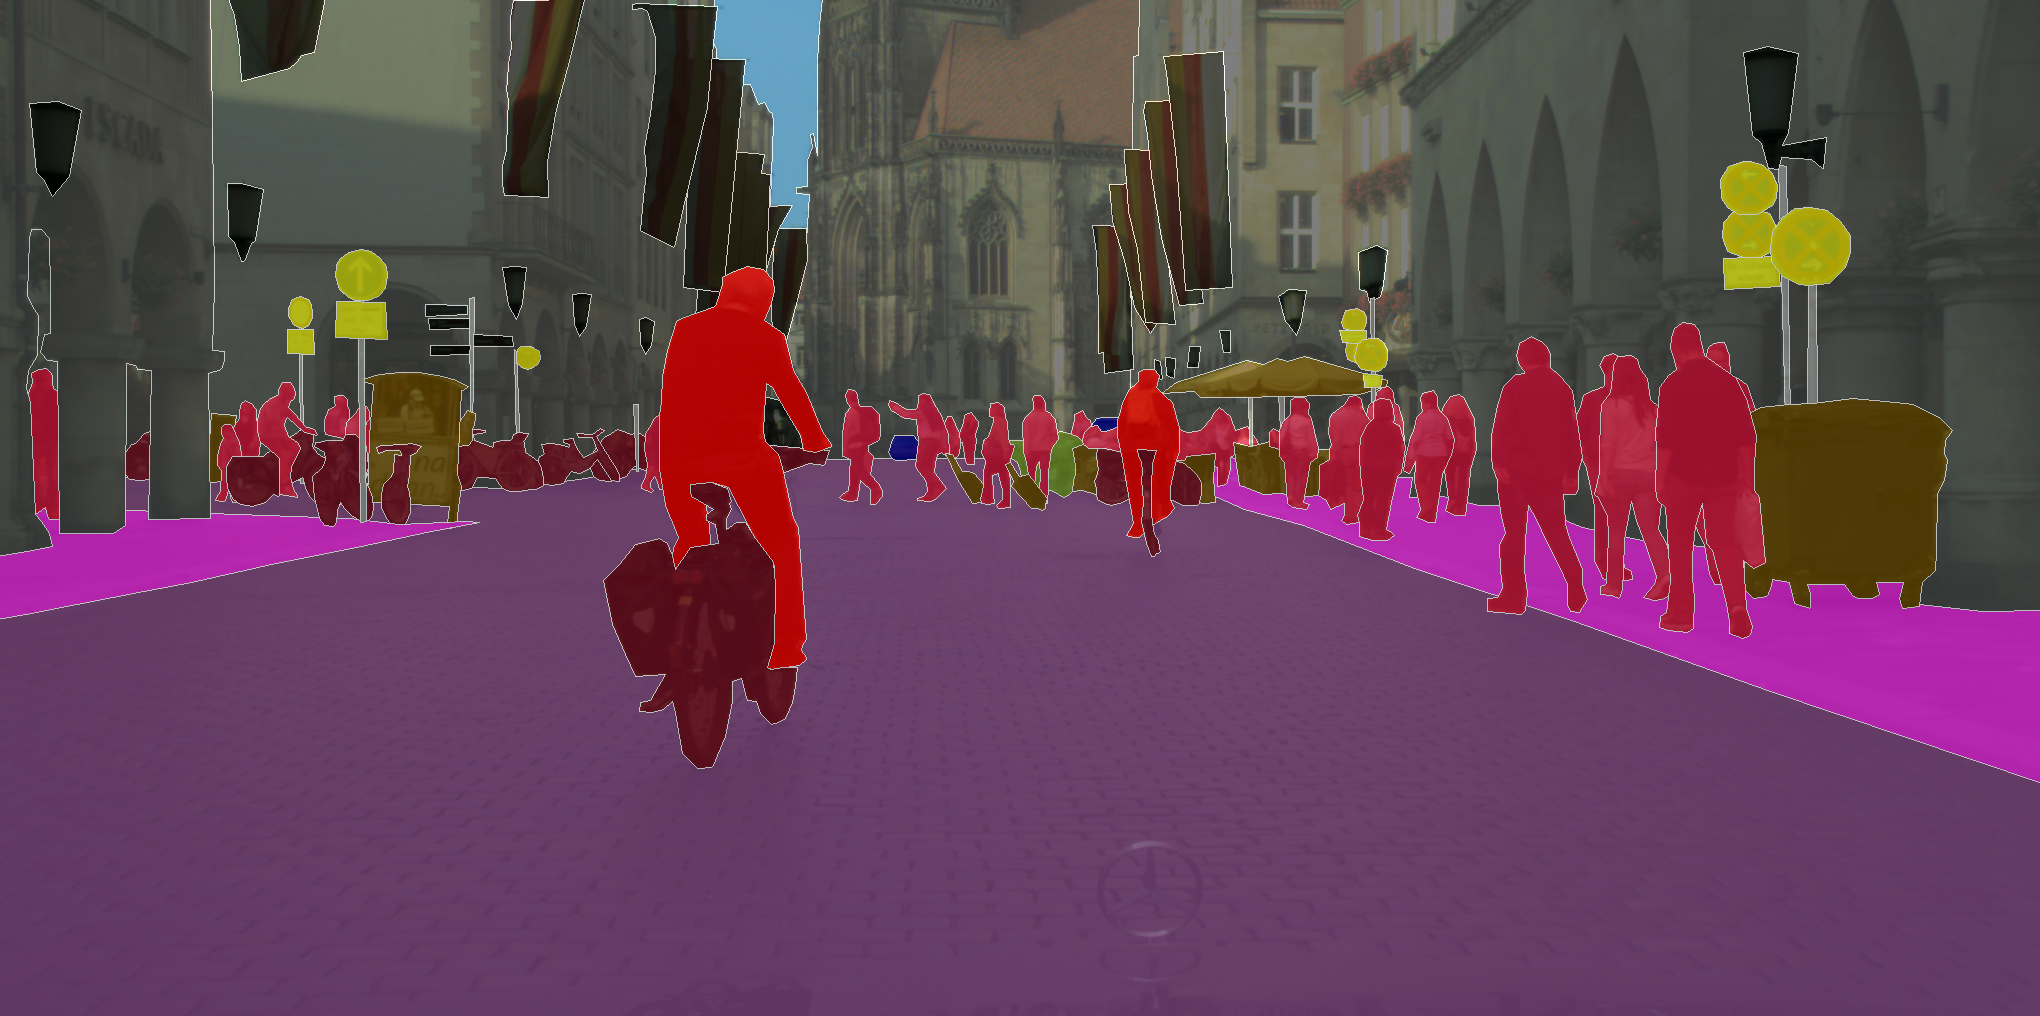
\includegraphics[width=0.6\textwidth]{cityscapes.png}
	\caption{Một kiểu gán nhãn trong Cityscapes}
	\label{fig:cityscapes}
\end{figure}
% \FloatBarrier

\footnotetext{\href{https://github.com/taintpro98/rnd-semantic-segmentation}{https://github.com/taintpro98/rnd-semantic-segmentation}}

\begin{table}[]
    \caption{Định nghĩa các lớp trong tập dữ liệu Cityscapes}
    \centering
    \begin{tabu} to \textwidth {|c|X[c]|}
        \hline
        \textbf{Nhóm} & \textbf{Các lớp tương ứng} \\ \hline
        flat & road · sidewalk · parking+ · rail track+ \\ \hline
        human & person* · rider* \\ \hline
        vehicle & car* · truck* · bus* · on rails* · motorcycle* · bicycle* · caravan*+ · trailer*+ \\ \hline
        construction & building · wall · fence · guard rail+ · bridge+ · tunnel+ \\ \hline
        object & pole · pole group+ · traffic sign · traffic light \\ \hline
        nature & vegetation · terrain \\ \hline
        sky & sky \\ \hline
        void & ground+ · dynamic+ · static+ \\ \hline
    \end{tabu}
    \label{tab:cityscapes}
\end{table}

\subsubsection{Bộ mô phỏng Carla}

Một hướng cải tiến của bài toán là ta áp dụng bộ mô phỏng Carla \cite{dosovitskiy2017carla} thêm dữ liệu cho tập nguồn, làm cho thông tin trở nên đa dạng và phong phú hơn. Thêm vào đó, dữ liệu được thêm vào không chỉ là cảnh đường phố ban ngày với đường khô ráo nữa mà còn được bổ sung thêm các kiểu thời tiết và thời gian khác như: trong cơn mưa, sau cơn mưa, bình minh, hoàng hôn, ban đêm, ... Đồ án thực hiện sinh ảnh từ bộ mô phỏng với 5 cấu hình được thể hiện trong Bảng \ref{tab:carla-config}

\begin{table}[]
    \caption{Cấu hình trong bộ sinh ảnh Carla}
    \centering
    \begin{tabu} {|c|c|c|c|c|}
        \hline
        \textbf{Cấu hình} & \textbf{Thời tiết} & \textbf{Số phương tiện} & \textbf{Số người} & \textbf{Bản đồ} \\ \hline
        1 & 1 (ClearNoon) & 100 & 300 & Thị trấn 1 \\ \hline
        2 & 8 (ClearSunset) & 100 & 50 & Thị trấn 1 \\ \hline
        3 & 2 (CloudyNoon) & 100 & 50 & Thị trấn 1 \\ \hline
        4 & 0 (Default) & 100 & 100 & Thị trấn 2 \\ \hline
        5 & 7 (SoftRainNoon) & 80 & 50 & Thị trấn 2 \\ \hline
    \end{tabu}
    \label{tab:carla-config}
\end{table}

Trong bộ mô phỏng Carla chỉ có 13 lớp. Trong đó nhãn "other" ta buộc phải bỏ qua vì thông tin của nó không cụ thể. Hoặc ví dụ như nhãn "vehicle" trong Carla quá chung chung bao gồm nhiều nhãn khác trong Cityscapes. Vậy nên, bộ mô phỏng Carla chỉ đóng vai trò làm giàu thêm cho một vài lớp sẵn có trong GTA5 chứ không thể hoàn toàn thay thế. Bù lại, nó đảm bảo cho sự đa dạng, tuỳ biến dữ liệu ảnh đường phố theo nhu cầu huấn luyện mà ta mong muốn. Cụ thể các lớp của Carla được thể hiện trong Bảng \ref{tab:carla} 

\begin{table}[]
    \caption{Định nghĩa các lớp trong tập dữ liệu được sinh từ Bộ mô phỏng Carla}
    \centering
    \begin{tabu} to \textwidth {|c|c|}
        \hline
        \textbf{Tên lớp} & \textbf{Giá trị RGB} \\ \hline
        None & 0, 0, 0 \\ \hline
        building & 0, 127, 180 \\ \hline
        fence & 127, 40, 127 \\ \hline
        other & 80, 180, 80 \\ \hline
        pedestrians & 255, 127, 127 \\ \hline
        pole & 180, 180, 180 \\ \hline
        roadline & 255, 180, 0 \\ \hline
        road & 255, 255, 0 \\ \hline
        sidewalk & 255, 0, 255 \\ \hline
        vegetation & 0, 255, 0 \\ \hline
        vehicle & 0, 0, 255 \\ \hline
        wall & 127, 40, 127 \\ \hline
        traffic sight & 255, 0, 0 \\ \hline
    \end{tabu}
    \label{tab:carla}
\end{table}

\subsubsection{Tương thích nhãn giữa các tập dữ liệu}

Một vấn đề cần lưu ý là sự tương thích về nhãn giữa các tập dữ liệu với nhau. Định nghĩa các lớp trong tập dữ liệu Cityscapes đã được thể hiện trong Bảng \ref{tab:cityscapes}. Nhưng trong tập GTA5 và Bộ mô phỏng Carla không thể có hết. Coi dữ liệu được sinh ra từ bộ mô phỏng Carla như dữ liệu tập nguồn bổ sung, ta có quy tắc tương thích nhãn các tập dữ liệu như sau:

\begin{itemize}
	\item Ta chỉ quan tâm đến 19 nhãn chung giữa GTA5 và Cityscapes. Chỉ huấn luyện và đánh giá mô hình trên 19 nhãn này. Gọi đây là tập "nhãn đích"
	\item Trên tập dữ liệu GTA5 và Cityscapes, nhãn nào không thuộc tập "nhãn đích" thì ta bỏ qua bằng cách gán cho nó giá trị là 255. Các nhãn còn lại, chuyển chúng về khoảng các số nguyên từ 0 đến 18 cho đồng bộ.
	\item Trên tập dữ liệu Carla, nhãn nào thuộc tập "nhãn đích" hoặc được bao hàm trong một nhãn thuộc "nhãn đích" thì sẽ được chuyển đổi tương ứng. Ví dụ như pedestrians được chuyển đổi thành person. Nếu nhãn nào bao hàm một nhãn trong tập "nhãn đích" thì ta có thể bỏ qua luôn bằng cách chuyển đổi nó thành 255. 
\end{itemize}

\section{Tiền xử lý dữ liệu}
Kích thước ảnh Cityscapes cần xử lý là 2048 x 1024. Tập dữ liệu của ta được chia làm 2 loại là tập nguồn (GTA5) và tập đích (Cityscapes). Ta sử dụng các phép biến đổi sau cho việc xử lý dữ liệu đầu vào:
\begin{itemize}
	\item Normalize: Chuẩn hoá một ảnh với giá trị trung bình và độ lệch chuẩn
	\item Horizonttal Flip: Lật ngược ảnh theo chiều ngang  
	\item Resize: Thay đổi kích thước của ảnh 
	\item Color Jitter: Thay đổi ngẫu nhiên độ sáng, độ tương phản, độ bão hòa và màu sắc của hình ảnh.
\end{itemize}

Trước khi bắt đầu huấn luyện, ta thực hiện xử lý dữ liệu như trong hình \ref{fig:preprocess}
\begin{figure}[htp]
	\centering
	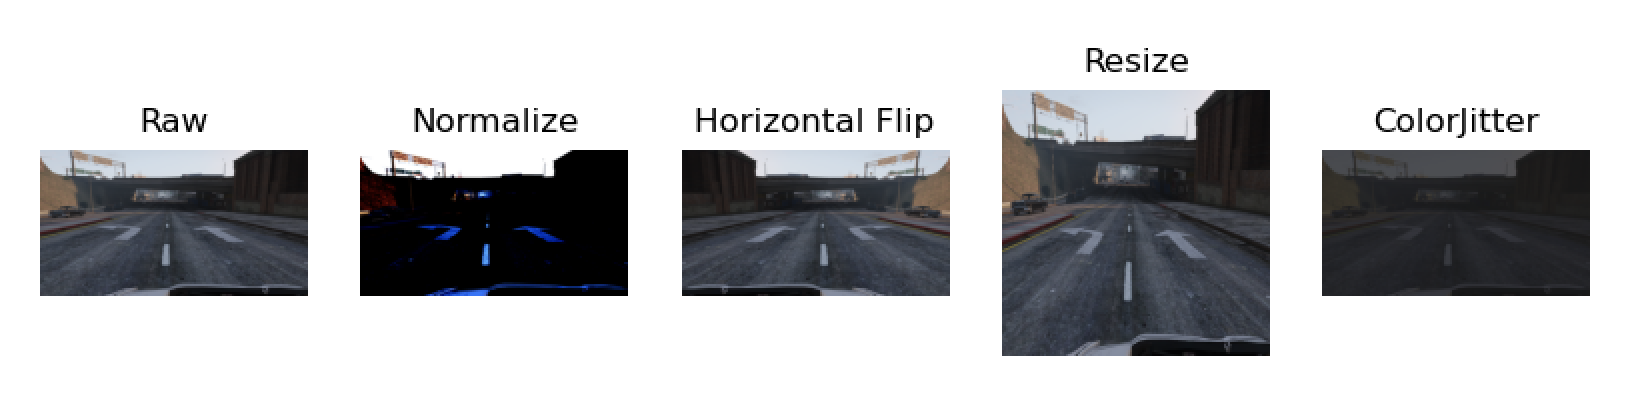
\includegraphics[width=1\textwidth]{preprocess.png}
	\caption{Tiền xử lý dữ liệu giúp cho mô hình học được những thông tin đa dạng hơn}
	\label{fig:preprocess}
\end{figure}

\section{Thiết lập thử nghiệm }
Trong bài toán này ta sử dụng mô hình Fine-grained Discriminator \cite{wang2020classes}. Việc huấn luyện mô hình này tương đối mất nhiều thời gian và đòi hỏi lượng dữ liệu lớn. Quá trình huấn luyện bao gồm 3 giai đoạn như đã nêu ở chương trước. Cùng với đó, chúng ta cần phải sử dụng các kỹ thuật tiền xử lý dữ liệu và lựa chọn các tham số phù hợp trong quá trình huấn luyện mô hình. Một vài hạn chế của mô hình hiện tại đó là:
\begin{itemize}
	\item Ở giai đoạn 1, mô hình chỉ được học từ dữ liệu nguồn nhằm tạo một mô hình cơ bản. Với những thông tin được cho từ tập nguồn, mô hình có thể học tốt nhưng chưa chắc đã khớp với thông tin trong tập đích.  
	\item Mô hình gặp hiện tượng quá khớp khi mà càng về các vòng cuối thì hàm mất mát tuy giảm nhưng hiệu năng lại không tăng tương ứng.
\end{itemize}

Những hạn chế này có thể ảnh hưởng đến kết quả cuối cùng của bài toán phân vùng ảnh. Một số kết quả thu được được minh hoạ trong (Hình \ref{fig:frankfurt_000000_005898_gtFine_labelIds}).
\begin{figure}[htp]
	\centering
	
\includegraphics[width=1\textwidth]{frankfurt_000000_005898_gtFine_labelIds.png}
	\caption{Theo thứ tự lần lượt là: Ảnh đầu vào, nhãn thật, kết quả sau giai đoạn 1, kết quả sau giai đoạn 2, kết quả sau giai đoạn 3}
	\label{fig:frankfurt_000000_005898_gtFine_labelIds}
\end{figure}
% \FloatBarrier

Tất cả các mô hình đều được thực hiện bằng: 
\begin{itemize}
	\item Pytorch 1.6.0 và CUDA 11.1
	\item Chạy trên 1 GPU Nvidia RTX3090 duy nhất
\end{itemize}

\subsection{Huấn luyện mô hình cơ sở trên tập dữ liệu nguồn}

Giai đoạn này mô hình được huấn luyện trên tập dữ liệu nguồn GTA5 bao gồm 22500 ảnh. Bao gồm 9 fold, mỗi fold là 2500 ảnh. Để lại fold thứ 10 để đánh giá khả năng học của mô hình trên tập dữ liệu nguồn. Ta sử dụng Cross Entropy làm hàm mất mát như đã trình bày ở chương trước (lưu ý là ta dùng ignore label bằng 255 để bỏ qua những nhãn không muốn huấn luyện). Bên cạnh đó, ta còn cần một chiến thuật cho tốc độ học hiệu quả. Ở đây, cả 2 mô hình đèu sử dụng hàm điều tiết tốc độ học là hàm mũ có công thức:

\begin{align}
& lr = base * (1 - \frac{i}{m})^{power}
\label{equa:power_lr}
\end{align}

Trong đó,
\begin{itemize}
	\item $lr$ là tốc độ học
	\item $base$ là tốc độ học khởi tạo
	\item $i$ là iteration hiện tại
	\item $m$ là iteration kết thúc
	\item $power$ là số mũ, ở đây ta chọn $power$ bằng 0.9
\end{itemize}

\subsubsection{Huấn luyện mô hình Resnet101 + DeeplabV2}

Hàm mất mát được tối ưu sử dụng thuật toán Stochastic gradient descent(SGD) với tốc độ học (learning rate) khởi tạo cho khối Encoder là 5e-4 và cho khối Decoder là 5e-3 được điều tiết sử dụng hàm mũ \ref{equa:power_lr}. Thuật toán huấn luyện trên 10 vòng và kích thước một batch là 6 (do kích thước ảnh khá lớn).

Sau 10 vòng huấn luyện, hàm mất mát từ 1.7370 dần hội tụ đến 0.1498. Hình \ref{fig:src_aspp_params}

\begin{figure}[htp]
	\centering
	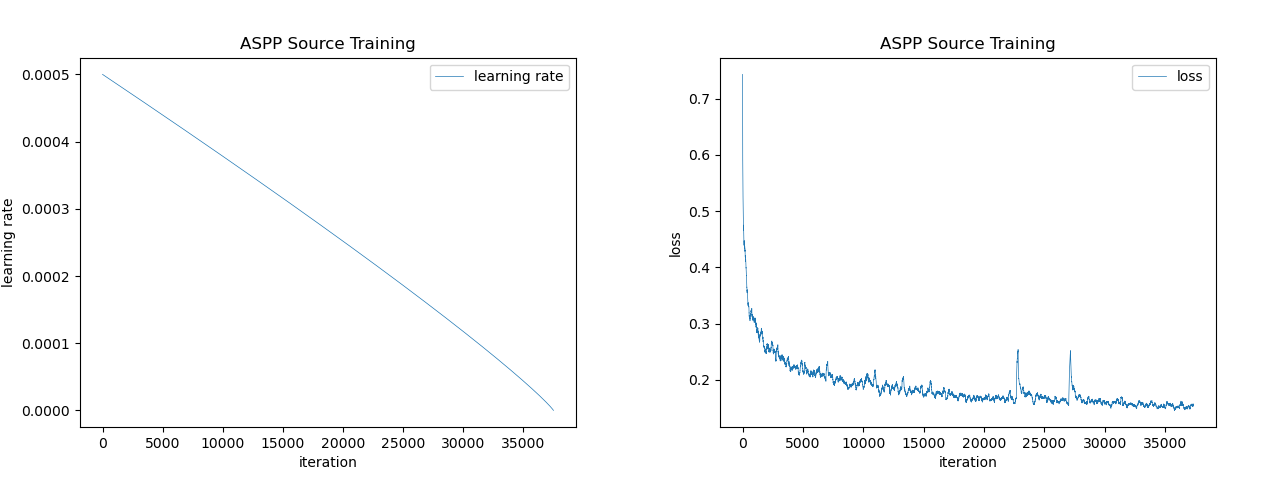
\includegraphics[width=1\textwidth]{images/src_aspp_params.png}
	\caption{Bên trái là kết quả tốc độ học qua các iteration. Bên phải là kết quả hàm mất mát trong quá trình huấn luyện Resnet101 + DeeplabV2 trên tập nguồn. Được đánh giá trên từng iteration, trong đó ta sử dụng trung bình động với kích thước cửa sổ là 150}
	\label{fig:src_aspp_params}
\end{figure}

\subsubsection{Huấn luyện mô hình Hardnet68 + GALD}

Hàm mất mát được tối ưu sử dụng thuật toán Adam với tốc độ học (learning rate) khởi tạo cho khối Encoder là $0.0001$ và cho khối Decoder là $0.001$ được điều tiết sử dụng hàm mũ \ref{equa:power_lr}. Thuật toán huấn luyện trên 10 vòng và kích thước một batch là 6 (do kích thước ảnh khá lớn).
Sau 10 vòng huấn luyện, hàm mất mát từ 1.8543 dần hội tụ đến 0.2757. Điều đó cho thấy mô hình này đã học rất tốt với các thông tin từ tập nguồn. Hình \ref{fig:src_gald_params} 

\begin{figure}[htp]
	\centering
	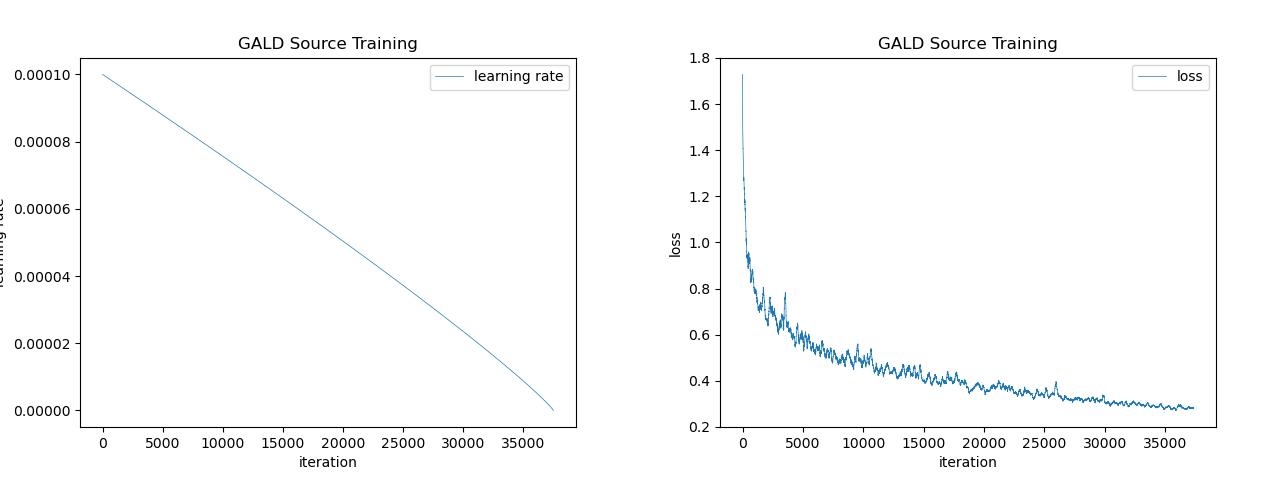
\includegraphics[width=1\textwidth]{images/src_gald_params.png}
	\caption{Bên trái là kết quả tốc độ học qua các iteration. Bên phải là kết quả hàm mất mát trong quá trình huấn luyện Hardnet68 + GALD trên tập nguồn. Được đánh giá trên từng iteration, trong đó ta sử dụng trung bình động với kích thước cửa sổ là 150}
	\label{fig:src_gald_params}
\end{figure}

\subsubsection{Huấn luyện mô hình Resnet101 + DeeplabV2 với tập dữ liệu nguồn bổ sung thêm Carla}

Ta giữ nguyên cấu hình các tham số như khi huấn luyện mô hình Resnet101 + DeeplabV2 bình thường nhưng trộn thêm dữ liệu được Carla sinh thêm với 22500 ảnh GTA5.

\subsection{Huấn luyện cạnh tranh trên tập dữ liệu trộn giữa tập nguồn và tập đích}

Ta đồng thời khởi tạo cả mô hình cơ sở và Bộ phân loại, cho chúng huấn luyện cùng lúc để cạnh tranh lẫn nhau. Trong đó, mô hình cơ sở vẫn giữ nguyên cấu hình như ở giai đoạn 1. Đối với Bộ phân loại, hàm mất mát được tối ưu sử dụng thuật toán Adam với tốc độ học là 0.0001 vẫn sử dụng hàm mũ để điều tiết. Thuật toán được huấn luyện trên 10 vòng với kích thước batch là 8 (4 ảnh nguồn và 4 ảnh đích). Ta nhắc lại vai trò của 4 hàm mất mát cùng được sử dụng trong giai đoạn này:
\begin{itemize}
	\item segmentation loss: tính toán sai số giữa kết quả do mô hình cơ sở dự đoán trên tập nguồn. 
	\item target adversarial loss: tính toán mức độ tương đồng giữa "tập đích" với "tập nguồn". Nghĩa là nếu như kết quả Bộ phân biệt dự đoán một ảnh thuộc "tập đích" càng giống với "tập nguồn" thì hàm mất mát này càng thấp.
	\item source disciminator loss và target discriminator loss: đo khả năng phân biệt một ảnh có thuộc đúng tập hợp của nó hay không. Tức là nếu như Bộ phân biệt dự đoán một ảnh trong đúng tập của nó thì hàm mất mát càng thấp.
\end{itemize}

\subsubsection{Huấn luyện cạnh tranh mô hình Resnet101 + DeeplabV2}

Sau 10 vòng huấn luyện:
\begin{itemize}
	\item segmentation loss từ 0.3263 dần hội tụ về 0.1568
	\item target adversarial loss không thay đổi nhiều, từ 0.0020 hội tụ về 0.0056. Nên ta thấy trong Hình \ref{fig:adv_aspp_params} thì hàm mất mát này gần như bằng 0 vì ta lấy trung bình động. 
	\item source disciminator loss từ 1.3027 hội tụ về 0.1658
	\item target discriminator loss từ 1.1807 hội tụ về 0.2205
\end{itemize}

\begin{figure}[htp]
	\centering
	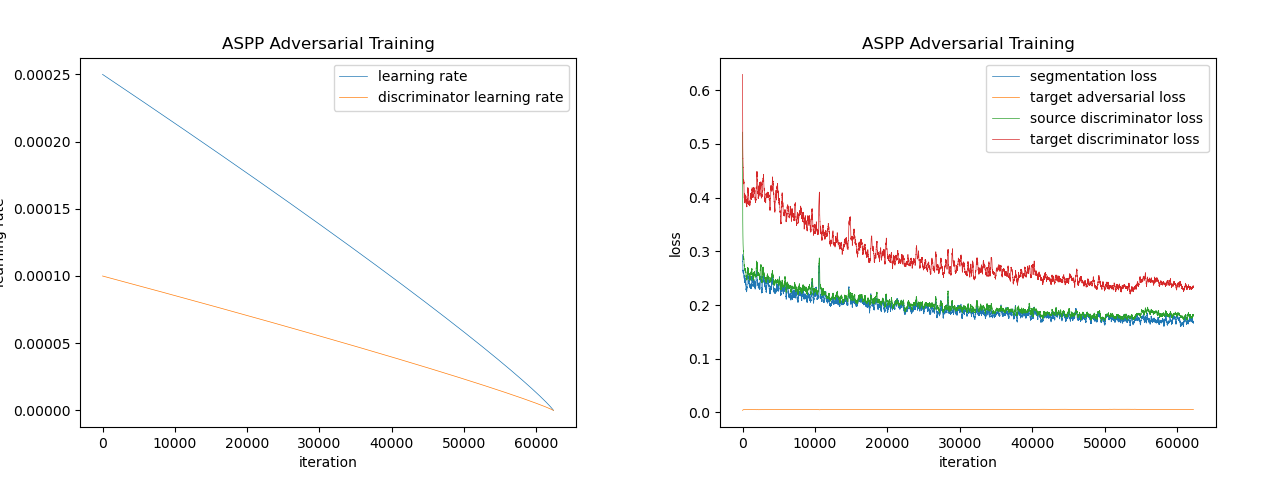
\includegraphics[width=1\textwidth]{images/adv_aspp_params.png}
	\caption{Bên trái là kết quả tốc độ học của mô hình cơ sở và bộ phân biệt qua các iteration. Bên phải là kết quả hàm mất mát trong quá trình huấn luyện cạnh tranh Resnet101 + DeeplabV2 trên tập nguồn trộn tập đích. Được đánh giá trên từng iteration, trong đó ta sử dụng trung bình động với kích thước cửa sổ là 150}
	\label{fig:adv_aspp_params}
\end{figure}

Sở dĩ giá trị của target adversarial loss lại nhỏ như vậy là do trọng số cho hàm mất mát này tác giả để rất nhỏ, chỉ $0.001$

\subsubsection{Huấn luyện cạnh tranh mô hình Hardnet68 + GALD}

Sau 10 vòng huấn luyện:
\begin{itemize}
	\item segmentation loss từ 0.1737 dần hội tụ về 0.0796
	\item target adversarial loss không thay đổi nhiều, từ 0.0023 hội tụ về 0.0054. Cũng tương tự như mô hình thứ nhât (như Hình \ref{fig:adv_gald_params}) thì hàm mất mát này gần như bằng 0 
	\item source disciminator loss từ 1.0428 hội tụ về 0.1615
	\item target discriminator loss từ 0.9669 hội tụ về 0.2058
\end{itemize}

\begin{figure}[htp]
	\centering
	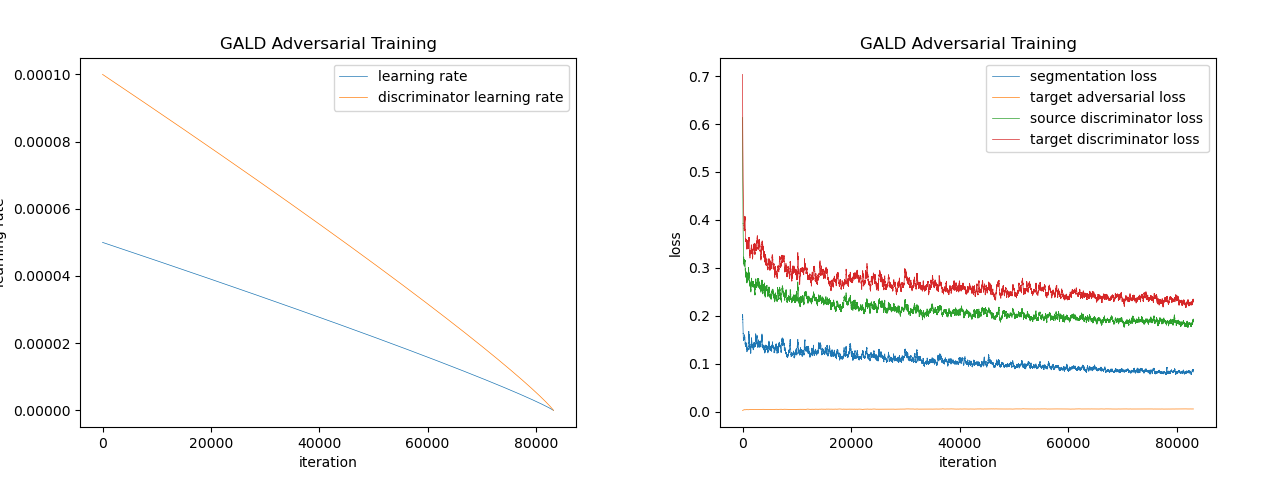
\includegraphics[width=1\textwidth]{images/adv_gald_params.png}
	\caption{Bên trái là kết quả tốc độ học của mô hình cơ sở và bộ phân biệt qua các iteration. Bên phải là kết quả hàm mất mát trong quá trình huấn luyện cạnh tranh Global Aggregate and Local Distribution trên tập nguồn trộn tập đích. Được đánh giá trên từng iteration, trong đó ta sử dụng trung bình động với kích thước cửa sổ là 150}
	\label{fig:adv_gald_params}
\end{figure}

So với mô hình thứ nhất, ta thấy rằng segmentation loss của mô hình Hardnet68 + GALD thấp hơn. Điều này thể hiện khả năng khớp dữ liệu nguồn của mô hình này rất tốt.

\subsection{Huấn luyện tự chắt lọc trên tập dữ liệu đích với nhãn giả được sinh từ giai đoạn 2}

Trước tiên, từ mô hình thu được ở giai đoạn 2, ta phải sinh ra tập các nhãn giả của bộ dữ liệu huấn luyện Cityscapes (vì mặc định coi như ta không có nhãn thật của Cityscapes). Nhãn giả được sinh ra tương tự minh hoạ trong Hình \ref{fig:frankfurt_000000_005898_gtFine_labelIds} (chính là kết quả sau giai đoạn 2). Các bước cấu hình huấn luyện và tham số không khác gì ở giai đoạn 1. Chỉ là thay đổi tập dữ liệu huấn luyện từ GTA5 thành tập Cityscapes với nhãn giả. Phương pháp này không làm tăng hiệu năng cho mô hình với kích thước huấn luyện là [1024, 512]. Nhưng khi kiểm thứ với kích thước gốc của ảnh trong tập kiểm thử là [2048, 1024] thì kết quả cải thiện lên rất tốt. Sự thay đổi được thể hiện trong Bảng \ref{tab:results}


% \begin{table}[]
%     \caption{Kết quả trên mô hình thứ nhất Resnet101 + DeeplabV2 đánh giá trên tập kiểm thử của Cityscapes}
%     \centering
%     \begin{tabu} to \textwidth {|c|X[c]|X[c]|X[c]|}
%         \hline
%         \textbf{Kích thước} & \textbf{Huấn luyện nguồn} & \textbf{Huấn luyện cạnh tranh} & \textbf{Tự cô đọng} \\ \hline
%         1024, 512 & 36.93 & 45.39 & 45.35 \\ \hline
%         2048, 1024 & 32.01 & 43.05 & 48.42 \\ \hline
%     \end{tabu}
%     \label{tab:deeplabv2}
% \end{table}

\section{Kết quả thực nghiệm}

\subsection{Sau khi học trên tập nguồn}

Ta có thể thấy rằng mô hình Hardnet68 + GALD khớp dữ liệu tốt hơn mô hình Resnet101 + DeeplabV2 do kết quả đánh giá trên tập huấn luyện là GTA5 tốt hơn tới 10 \%. Nhưng khi đánh giá trên tập Cityscapes thì mô hình Resnet101 + DeeplabV2 lại tốt hơn 4 \%. Điều này cho thấy rằng việc quá khớp với dữ liệu nguồn đã làm cho mô hình Hardnet68 + GALD trở nên kém tổng quát hơn. Trong khi đó, việc thêm dữ liệu Carla vào tập nguồn mặc dù làm giảm đi khả năng học của mô hình Resnet101 + DeeplabV2 nhưng đã giúp đa dạng hoá dữ liệu hơn và đạt được hiệu năng tốt nhất trong 3 hướng tiếp cận. Bảng \ref{tab:phase1}

\begin{table}[]
    \caption{So sánh kết quả trên mô hình Resnet101 + DeeplabV2 và mô hình Hardnet68 + GALD đánh giá trên fold thứ 10 của tập GTA5 và tập kiểm thử của Cityscapes với kích thước đầu vào là [1024, 512]}
    \centering
    \begin{tabu} to \textwidth {|c|X[c]|X[c]|}
        \hline
        \textbf{Mô hình} & \textbf{Tập dữ liệu GTA5} & \textbf{Tập dữ liệu Cityscapes} \\ \hline
        Resnet101 + DeeplabV2 & 67.88 & 36.93 \\ \hline
        Hardnet68 + GALD & 77.54 & 32.17 \\ \hline
        Resnet101 + DeeplabV2 (+Carla) & 60.87 & 37.76 \\ \hline
    \end{tabu}
    \label{tab:phase1}
\end{table}

\subsection{Sau khi học cạnh tranh}

Sau khi huấn luyện cạnh tranh thì kết quả trên tập kiểm thử của Cityscapes đều tăng gần 10 \% với mỗi mô hình. Ta thấy rằng kết quả ở giai đoạn 1 của mô hình rất quan trọng đối với việc huấn luyện ở giai đoạn 2. Mặc dù mô hình Hardnet68 + GALD đã khớp dữ liệu GTA5 tốt hơn hẳn Resnet101 + DeeplabV2 nhưng lại thua kém khi đánh giá trên tập kiểm thử Cityscapes. Điều đó dẫn đến khi huấn luyện giai đoạn 2, mô hình Hardnet68 + GALD đã không đạt hiệu năng tốt như mô hình Resnet101 + DeeplabV2. Mặc dù, mô hình Resnet101 + DeeplabV2 chỉ tăng 8.46 \% còn mô hình Hardnet68 + GALD tăng những 10.71 \%. Ta cũng thấy rằng khi thêm dữ liệu Carla vào tập nguồn để huấn luyện thì hiệu năng sau giai đoạn 2 lại không tăng nhiều, chỉ tăng 6.38 \%. Bảng \ref{tab:phase2}

\begin{table}[]
    \caption{So sánh kết quả mô hình Resnet101 + DeeplabV2 và mô hình Hardnet68 + GALD đánh giá trên tập kiểm thử của Cityscapes với kích thước đầu vào là [1024, 512]}
    \centering
    \begin{tabu} to \textwidth {|c|X[c]|X[c]|}
        \hline
        \textbf{Mô hình} & \textbf{Sau khi huấn luyện nguồn} & \textbf{Sau khi huấn luyện cạnh tranh} \\ \hline
        Resnet101 + DeeplabV2 & 36.93 & 45.39\\ \hline
        Hardnet68 + GALD & 32.17 & 42.88 \\ \hline
        Resnet101 + DeeplabV2 (+Carla) & 37.76 & 44.14 \\ \hline
    \end{tabu}
    \label{tab:phase2}
\end{table}

\subsection{Sau khi học tự chắt lọc}

Ta nhận thấy rằng các phương pháp tiếp cận mới mặc dù làm tăng hiệu năng của mô hình trên tập GTA5 và trên tập kiểm thử của Cityscapes khi ở giai đoạn 1. Nhưng ở giai đoạn 2, thì mô hình Resnet101 + DeeplabV2 vẫn đạt hiệu quả cao nhất. Do đó, ta dùng mô hình này như một "giáo viên" để sinh "nhãn giả" cho các mô hình "sinh viên" học tập. Khi đó, mô hình "sinh viên" Hardnet68 + GALD đạt được hiệu năng cao nhất là 48.9 \%. 
Sau khi áp dụng các hướng tiếp cận trên, ta thu được kết quả như trong Bảng \ref{tab:results}

% \begin{table}[htp]
%     \centering
%     \caption{Bảng so sánh kết quả các mô hình trên 2 tập dữ liệu GTA5 và Cityscapes}
%     \begin{tabu} to \textwidth {|c|X[c]|X[c]|X[c]|X[c]|}
%         \hline
%          & \multicolumn{2}{c|}{\textbf{GTA5}} & \multicolumn{2}{c|}{\textbf{Cityscapes}} \\ \cline{2-5}
%          & \textbf{Kích thước (1024, 512)} & \textbf{Kích thước (2048, 1024)} & \textbf{Kích thước (1024, 512)} & \textbf{Kích thước (2048, 1024)} \\ \hline
%         Resnet101 + DeeplabV2 & 0.6788 & 0.6980 & 0.3693 & 0.3201\\ \hline
%         Resnet101 + DeeplabV2 (+Carla)& 0.6087 & 0.6176 & 0.3776 & 0.3515\\ \hline
%         Hardnet68 + GALD & \textbf{0.7754} & 0.7859 & 0.3217 & 0.2703 \\ \hline
%         Resnet101 + DeeplabV2 + Adv & 0.6839 & 0.7129 & \textbf{0.4539} & 0.4305 \\ \hline
%         Resnet101 + DeeplabV2 + Adv(+Carla)& Not yet & Not yet & 0.4414 & Not yet \\ \hline
%         Hardnet68 + GALD + Adv & Not yet & Not yet & 0.4288 & Not yet \\ \hline
%         Resnet101 + DeeplabV2 + Distill & Not yet & Not yet & 0.4535 & 0.4842 \\ \hline
%         Hardnet68 + GALD + Distill & Not yet & Not yet & Not yet & \textbf{48.90} \\ \hline
%     \end{tabu}
%     \label{tab:results}
% \end{table}
% \FloatBarrier

\begin{table}[htp]
    \centering
    \caption{Bảng so sánh kết quả các mô hình trên 2 tập dữ liệu GTA5 và Cityscapes}
    \begin{tabu} to \textwidth {|c|X[c]|X[c]|X[c]|X[c]|}
        \hline
         & \multicolumn{2}{c|}{\textbf{GTA5}} & \multicolumn{2}{c|}{\textbf{Cityscapes}} \\ \cline{2-5}
         & \textbf{Kích thước (1024, 512)} & \textbf{Kích thước (2048, 1024)} & \textbf{Kích thước (1024, 512)} & \textbf{Kích thước (2048, 1024)} \\ \hline
        Resnet101 + DeeplabV2 & 0.6788 & 0.6980 & 0.3693 & 0.3201\\ \hline
        Resnet101 + DeeplabV2 (+Carla)& 0.6087 & 0.6176 & 0.3776 & 0.3515\\ \hline
        Hardnet68 + GALD & \textbf{0.7754} & \textbf{0.7859} & 0.3217 & 0.2703 \\ \hline
        Resnet101 + DeeplabV2 + Adv & 0.6839 & 0.7129 & \textbf{0.4539} & 0.4305 \\ \hline
        Resnet101 + DeeplabV2 + Adv(+Carla)& 0.6566 & 0.6312 & 0.4414 & 0.4323 \\ \hline
        Hardnet68 + GALD + Adv & 0.6723 & 0.6428 & 0.4288 & 0.4112 \\ \hline
        Resnet101 + DeeplabV2 + Distill & 0.6639 & 0.6514 & 0.4535 & 0.4842 \\ \hline
        Hardnet68 + GALD + Distill & 0.7428 & 0.7219 & 0.4546 & \textbf{0.4890} \\ \hline
    \end{tabu}
    \label{tab:results}
\end{table}
\FloatBarrier
mIoU cho mô hình Hardnet68 + GALD với kích thước đầu vào [2048, 1024] là 48.9 \%. Ta minh hoạ kết quả bằng một confusion matrix như Hình \ref{fig:aspp_cmt}

\begin{figure}[htp]
	\centering
	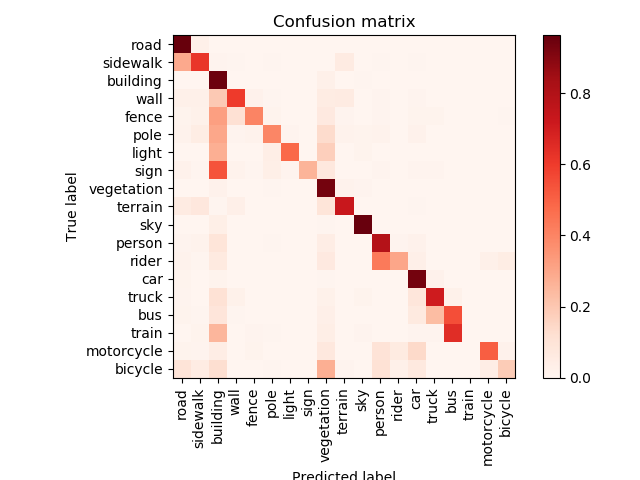
\includegraphics[width=0.9\textwidth]{images/aspp_cmt.png}
	\caption{Minh hoạ Confusion Matrix cho kết quả của mô hình Hardnet68 + GALD}
	\label{fig:aspp_cmt}
\end{figure}

Ta có một số nhận xét: 
\begin{itemize}
	\item (Hàng 2) sidewalk thường bị nhầm thành road 
	\item (Cột 3) nhiều lớp bị nhầm với lớp building, do mô hình không có khả năng trích xuất các vật thể nhỏ (light, pole, sign,…) khỏi nền có building
	\item Giao điểm của hàng 12-13 (person - rider) với cột 12-13 (person - rider): phân loại sai của mô hình giữa hai lớp này là dễ hiểu vì chúng không khác nhau trong thực tế.
\end{itemize}